

\begin{frame}{About me}
    \begin{itemize}
        \item Name: Lifeng Ren-2nd Year Ph.D. student in APEC.
        \begin{itemize}
            \item Call me Lifeng is fine. 
            \item Pronounced as "Lee-Phone".
        \end{itemize} 
        \item Education: 
        \begin{itemize}
            \item BS: Purdue: Math+Ag Econ
            \item MS: UC Davis: Applied Math+Ag Econ
        \end{itemize}
        \item Research: Environmental and Resource Economics
        \item Fun Facts about me outside of school: 
        
        \begin{itemize}
            \item Hometown: Nanjing, China 
            \item Favoratie Food: Nanjing Duck
            \begin{itemize}
                \item Roasted: 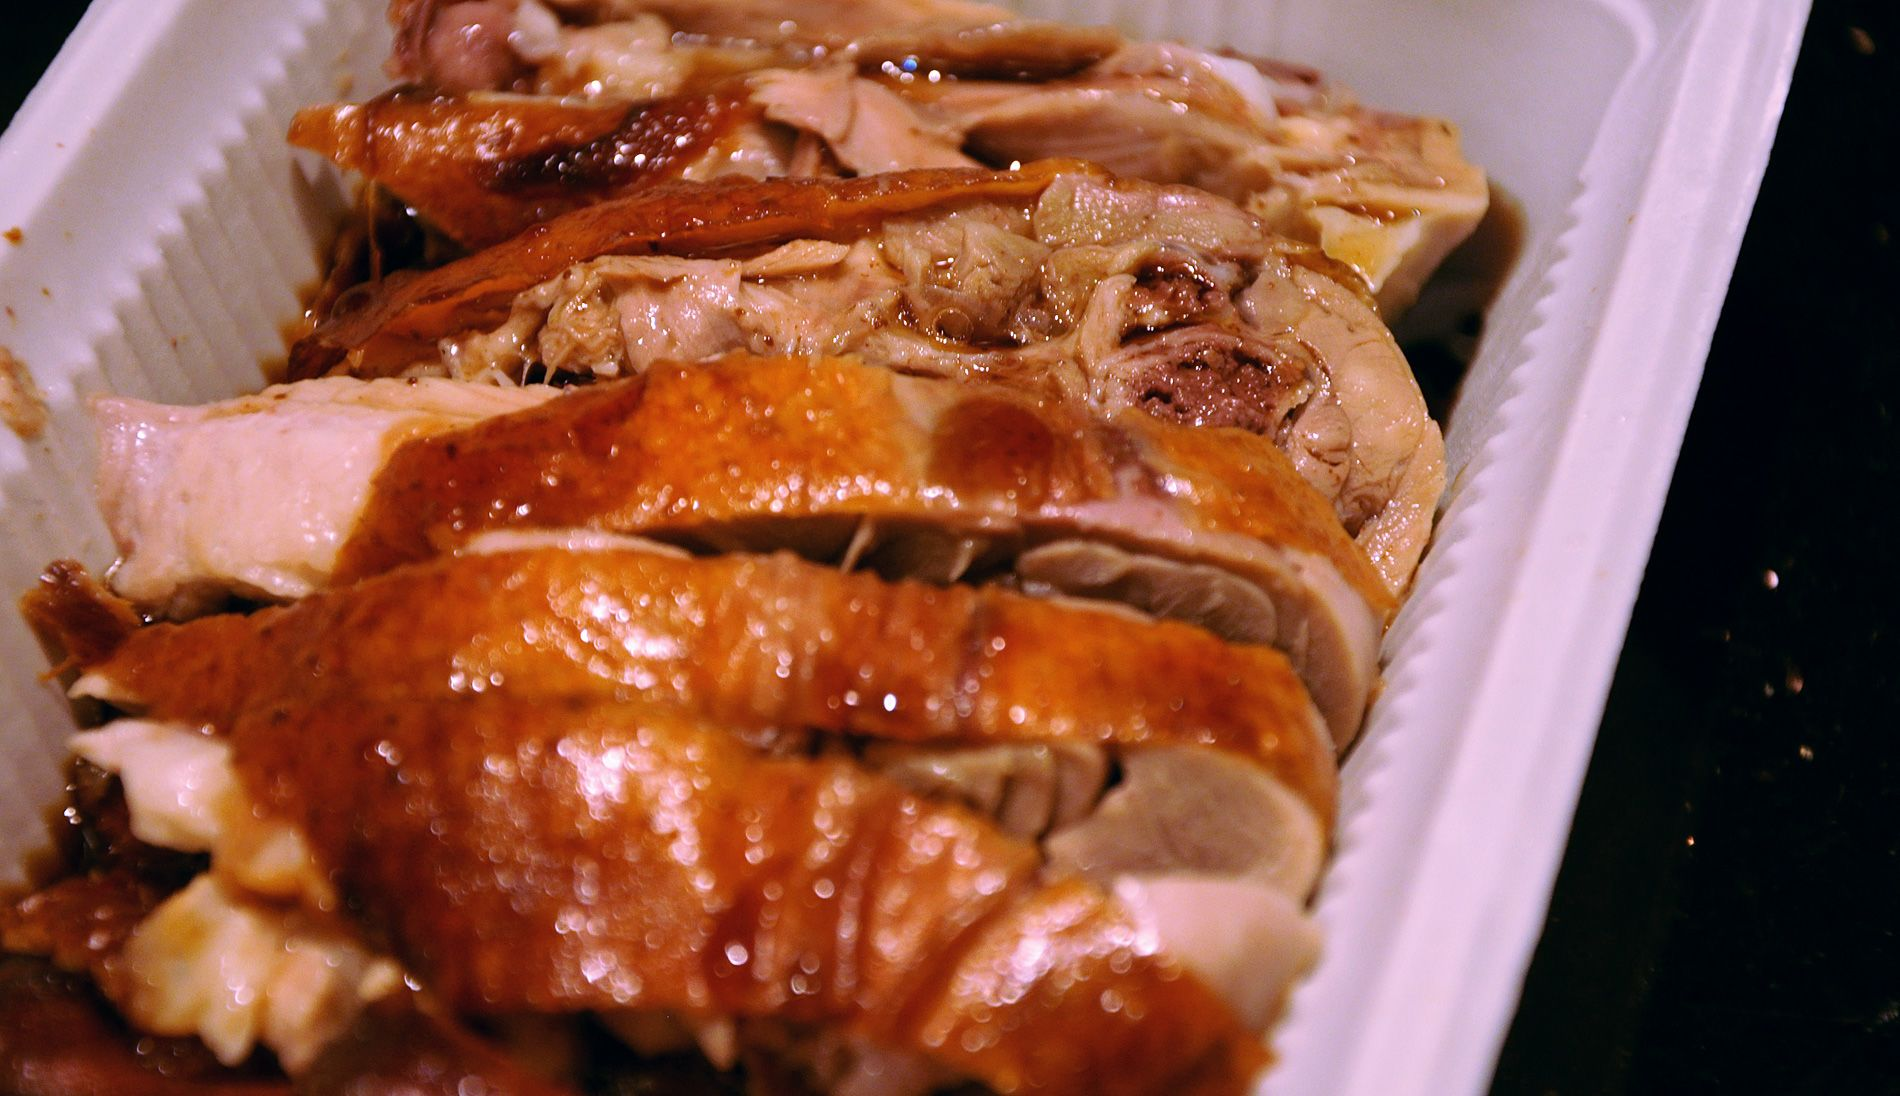
\includegraphics[width=1.8cm]{lec/nanjing_duck_roast.png}
                \item Salted: 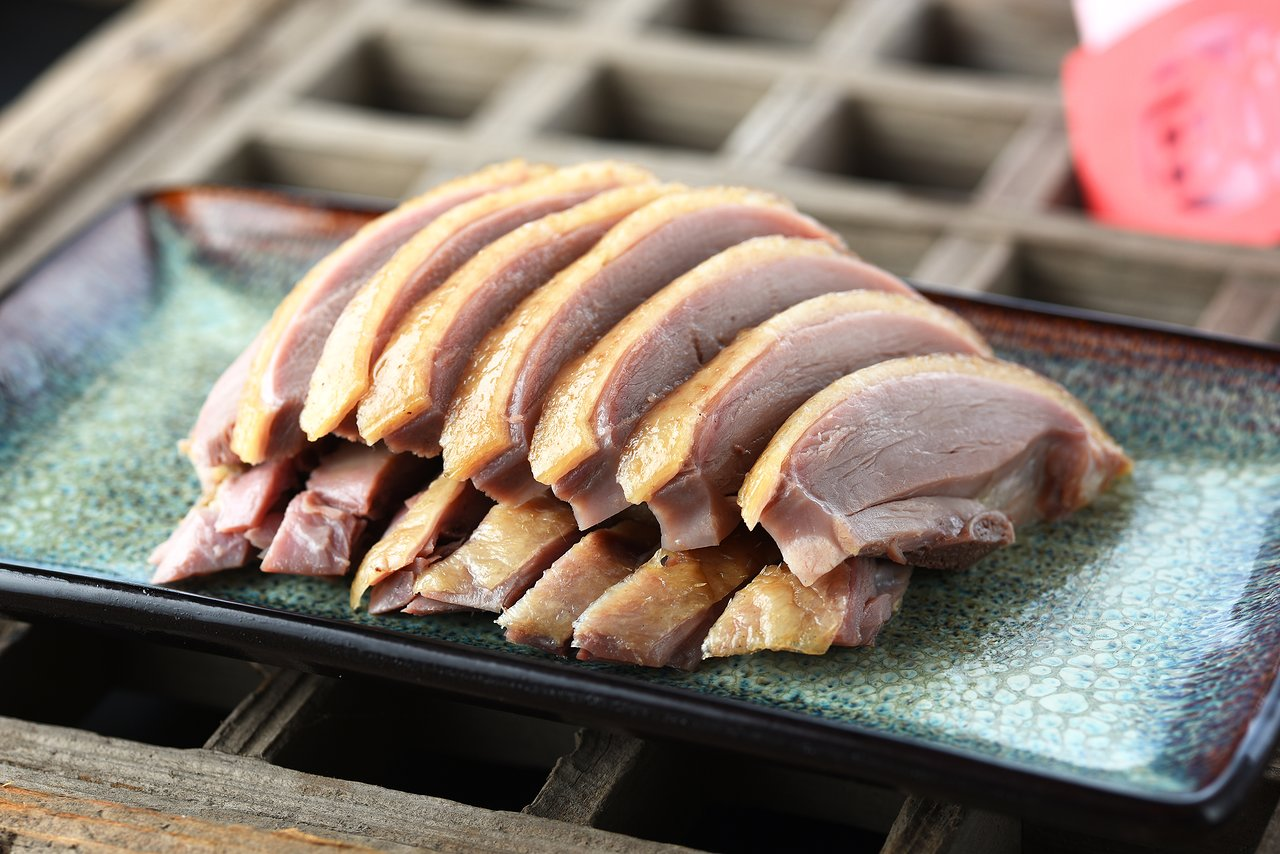
\includegraphics[width=1.8cm]{lec/nanjing_duck_salt.png}
            \end{itemize}
            
            
        \end{itemize}
        
    \end{itemize}
\end{frame}

\begin{frame}{About you}
Welcome! Let's Get to Know Each Other!
    \begin{itemize}
        \item What is your Name and Program?
        \item What are your research interests? 
        \item Fun Fact about you outside of school
        \item What do you expect to learn from this class? 
        \item Anything you would like to share with us more... 
    \end{itemize}
\end{frame}

\begin{frame}{About This Class}
\begin{itemize}
    \item We're on a journey to explore R together. Don't hesitate to ask if you're unsure about anything.
    \item Let's create a supportive, respectful learning space where we can all grow.
    \item Remember, mastering coding takes time and patience. I'm here for you, offering daily 1 hour office hour for extra help after our class. 
    \item 10 minutes break every hour.
    \item If possible, attending in person can be beneficial, especially if you're new to R. But remember, it's important to balance your studies and take breaks when needed, especially for those who are taking Math-review class at the same time. Your well-being matters! 
\end{itemize}

\end{frame}

\begin{frame}{Class Materials}
\begin{itemize}
    \item Syllabus and all other lecture-related materials are open-sourced and are provided on GitHub with this \href{https://github.com/lfr00154/R-review2023}{\underline{link}}. Feel free to use it for your own purpose. 
    \item The lectures will be recorded.
    \item Since everything will be open-sourced, you can study the materials at your own pace, and please let me know if there are any errors anywhere. 
\end{itemize}
    
\end{frame}

\begin{frame}{Switch to: GitHub} 
    \begin{itemize}
        \item Go to the repository: https://github.com/lfr00154/R-review2023
        \item Go over the repository structure.
        \item Download the folder for lec0 and lec1.
    \end{itemize}
\end{frame}

\begin{frame}{Today's Goal} 
    \begin{itemize}
        \item Get familiar with R and Rstudio.
        \item Data type and Data structure.
        \item If we have more time: Other tools that I think is useful for PhD study.
    \end{itemize}
\end{frame}

\begin{frame}[fragile]
    \Large Questions? 
\end{frame}

